% ===========================================================================
%  TikuOS — Memory Management: Persistent FRAM Key-Value Store
%  Beamer Presentation
% ===========================================================================
\documentclass[aspectratio=169, 10pt]{beamer}

% ---- Theme ----------------------------------------------------------------
\usetheme{Madrid}
\usecolortheme{whale}
\setbeamertemplate{navigation symbols}{}
\setbeamertemplate{footline}{%
  \leavevmode\hbox{%
    \begin{beamercolorbox}[wd=.33\paperwidth,ht=2.5ex,dp=1ex,center]{author in head/foot}%
      \usebeamerfont{author in head/foot}\insertshortauthor
    \end{beamercolorbox}%
    \begin{beamercolorbox}[wd=.34\paperwidth,ht=2.5ex,dp=1ex,center]{title in head/foot}%
      \usebeamerfont{title in head/foot}\insertshorttitle
    \end{beamercolorbox}%
    \begin{beamercolorbox}[wd=.33\paperwidth,ht=2.5ex,dp=1ex,right]{date in head/foot}%
      \usebeamerfont{date in head/foot}\insertshortdate{}\hspace*{2em}%
      \insertframenumber{}/\inserttotalframenumber\hspace*{2ex}
    \end{beamercolorbox}}%
  \vskip0pt%
}

% ---- Packages -------------------------------------------------------------
\usepackage{listings}
\usepackage{graphicx}
\usepackage{hyperref}
\usepackage{booktabs}
\usepackage{multirow}
\usepackage{tikz}
\usetikzlibrary{arrows.meta, positioning, shapes.geometric, calc, decorations.pathreplacing}

% ---- Code listing style ---------------------------------------------------
\lstset{
  basicstyle=\ttfamily\scriptsize,
  keywordstyle=\color{blue}\bfseries,
  commentstyle=\color{gray},
  stringstyle=\color{red!70!black},
  showstringspaces=false,
  breaklines=true,
  frame=single,
  rulecolor=\color{black!30},
  backgroundcolor=\color{blue!3},
  tabsize=4,
}
\lstdefinestyle{cstyle}{
  language=C,
  morekeywords={uint8_t,uint16_t,uint32_t,tiku_persist_store_t,
                tiku_persist_entry_t,tiku_mem_err_t,tiku_mem_arch_size_t,
                TIKU_MEM_OK,TIKU_MEM_ERR_INVALID,TIKU_MEM_ERR_NOMEM,
                TIKU_MEM_ERR_FULL,TIKU_MEM_ERR_NOT_FOUND,
                TIKU_PERSIST_MAGIC,TIKU_PERSIST_MAX_ENTRIES,
                TIKU_PERSIST_MAX_KEY_LEN,TIKU_PERSIST_WEAR_THRESHOLD,
                NULL},
}
\lstdefinestyle{bashstyle}{
  language=bash,
  morekeywords={sudo,apt,make,gcc},
}

% ---- Metadata -------------------------------------------------------------
\title[TikuOS Persistent Store]{TikuOS Persistent FRAM Key-Value Store}
\subtitle{Simple. Ubiquitous. Intelligence, Everywhere.}
\author[Ambuj Varshney]{Ambuj Varshney \\ \texttt{ambuj@tiku-os.org}}
\date{\today}

% ===========================================================================
\begin{document}

% ---------------------------------------------------------------------------
\begin{frame}
\titlepage
\end{frame}

% ---------------------------------------------------------------------------
\begin{frame}{Outline}
\tableofcontents
\end{frame}

% ===========================================================================
\section{Why Persistent Storage?}
% ===========================================================================

\begin{frame}{The Problem: Managing Non-Volatile Data on MCUs}
\begin{columns}[T]
\begin{column}{0.48\textwidth}
\textbf{Common approaches (and their issues):}
\begin{itemize}
  \item Raw FRAM writes scattered across code
  \item No validation after reboot --- FRAM garbage looks like real data
  \item No wear tracking --- silent degradation over years
  \item Firmware updates lose calibration data
  \item No consistent API for persistent config
\end{itemize}

\vspace{0.5em}
\begin{alertblock}{FRAM Is Not Free}
FRAM retains data across reboots, but has finite write endurance
(\textasciitilde$10^{15}$ cycles). Untracked hot writes can degrade cells
over the device lifetime.
\end{alertblock}
\end{column}

\begin{column}{0.48\textwidth}
\textbf{TikuOS persistent store:}
\begin{itemize}
  \item Registry of key $\rightarrow$ FRAM buffer mappings
  \item Magic number validates entries across reboots
  \item Write-count tracking for wear monitoring
  \item Re-registration preserves data across firmware updates
  \item All buffers statically declared --- zero dynamic allocation
\end{itemize}

\vspace{0.5em}
\begin{block}{Ideal Use Cases}
Device configuration, sensor calibration, boot counters,
error logs, operational state that must survive power loss.
\end{block}
\end{column}
\end{columns}
\end{frame}

% ===========================================================================
\section{Architecture \& Data Structures}
% ===========================================================================

\begin{frame}[fragile]{Persistent Entry Structure}
\begin{columns}[T]
\begin{column}{0.50\textwidth}
\begin{lstlisting}[style=cstyle, title={kernel/memory/tiku\_mem.h}]
typedef struct {
    char      key[TIKU_PERSIST_MAX_KEY_LEN];
    uint8_t  *fram_ptr;
    tiku_mem_arch_size_t value_len;
    tiku_mem_arch_size_t capacity;
    uint32_t  write_count;
    uint32_t  magic;
    uint8_t   valid;
} tiku_persist_entry_t;
\end{lstlisting}
\end{column}

\begin{column}{0.46\textwidth}
\begin{tabular}{@{}lp{4.2cm}@{}}
\toprule
\textbf{Field} & \textbf{Purpose} \\
\midrule
\texttt{key}          & Short string identifier \\
\texttt{fram\_ptr}    & Caller-provided FRAM buffer \\
\texttt{value\_len}   & Current stored data length \\
\texttt{capacity}     & Maximum buffer size \\
\texttt{write\_count} & Writes for wear tracking \\
\texttt{magic}        & 0x544B5553 if valid \\
\texttt{valid}        & Non-zero if entry is live \\
\bottomrule
\end{tabular}
\end{column}
\end{columns}

\vspace{0.5em}
\begin{block}{Key Design}
The store \textbf{does not own} the FRAM buffers --- the application provides
statically-declared FRAM regions. The store only manages the registry of
mappings and metadata.
\end{block}
\end{frame}

% ---------------------------------------------------------------------------
\begin{frame}[fragile]{Store Structure \& Constants}
\begin{columns}[T]
\begin{column}{0.48\textwidth}
\begin{lstlisting}[style=cstyle, title={Store control block}]
typedef struct {
    tiku_persist_entry_t
        entries[TIKU_PERSIST_MAX_ENTRIES];
    tiku_mem_arch_size_t count;
} tiku_persist_store_t;
\end{lstlisting}

\begin{lstlisting}[style=cstyle, title={Compile-time constants}]
/* Max entries (default 16) */
#define TIKU_PERSIST_MAX_ENTRIES  16

/* Max key length including \0 */
#define TIKU_PERSIST_MAX_KEY_LEN  8

/* Magic: "TKUS" in ASCII hex */
#define TIKU_PERSIST_MAGIC  0x544B5553U

/* Wear warning threshold */
#define TIKU_PERSIST_WEAR_THRESHOLD \
    1000000000UL
\end{lstlisting}
\end{column}

\begin{column}{0.48\textwidth}
\begin{lstlisting}[style=cstyle, title={Extended error codes}]
typedef enum {
    TIKU_MEM_OK          =  0,
    TIKU_MEM_ERR_INVALID = -1,
    TIKU_MEM_ERR_NOMEM   = -2,
    TIKU_MEM_ERR_FULL    = -3,
    TIKU_MEM_ERR_NOT_FOUND = -4
} tiku_mem_err_t;
\end{lstlisting}

\vspace{0.5em}
\begin{block}{Configurability}
All constants can be overridden with \texttt{\#define} before including
\texttt{tiku\_mem.h}. A constrained device might use
\texttt{MAX\_ENTRIES=4} and \texttt{MAX\_KEY\_LEN=4}.
\end{block}
\end{column}
\end{columns}
\end{frame}

% ---------------------------------------------------------------------------
\begin{frame}[fragile]{How Validation Works Across Reboots}
\begin{center}
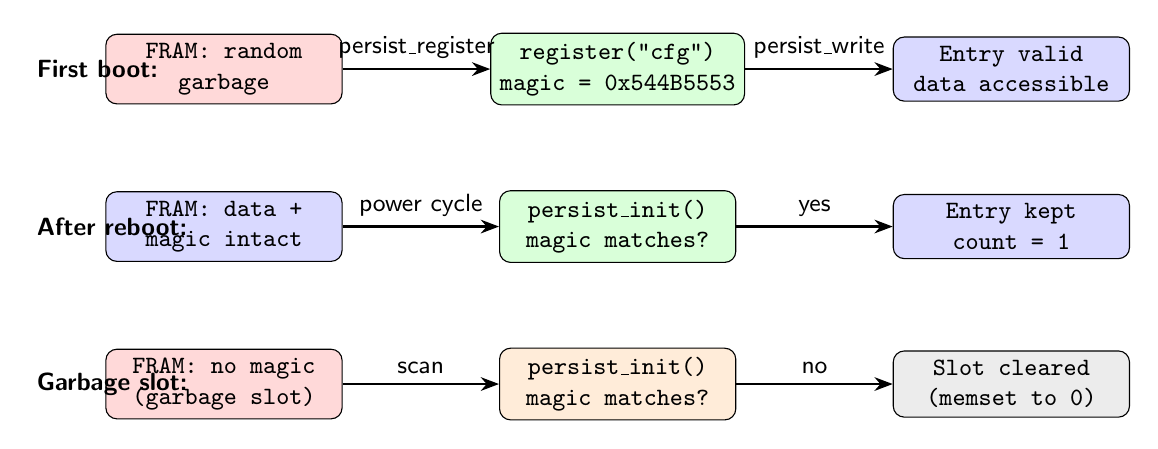
\begin{tikzpicture}[
    box/.style={draw, rounded corners, minimum width=3cm, minimum height=0.8cm,
                font=\small\ttfamily, align=center},
    label/.style={font=\small\sffamily},
    >=Stealth
  ]

  % First boot
  \node[box, fill=red!15] (raw) at (0, 2) {FRAM: random\\garbage};
  \node[box, fill=green!15] (reg) at (5, 2) {register("cfg")\\magic = 0x544B5553};
  \node[box, fill=blue!15] (valid) at (10, 2) {Entry valid\\data accessible};
  \draw[->, thick] (raw) -- (reg) node[midway, above, font=\small\sffamily] {persist\_register};
  \draw[->, thick] (reg) -- (valid) node[midway, above, font=\small\sffamily] {persist\_write};

  \node[label, anchor=west] at (-2.5, 2) {\textbf{First boot:}};

  % Reboot
  \node[box, fill=blue!15] (fram2) at (0, 0) {FRAM: data +\\magic intact};
  \node[box, fill=green!15] (init2) at (5, 0) {persist\_init()\\magic matches?};
  \node[box, fill=blue!15] (keep) at (10, 0) {Entry kept\\count = 1};
  \draw[->, thick] (fram2) -- (init2) node[midway, above, font=\small\sffamily] {power cycle};
  \draw[->, thick] (init2) -- (keep) node[midway, above, font=\small\sffamily] {yes};

  \node[label, anchor=west] at (-2.5, 0) {\textbf{After reboot:}};

  % Bad entry
  \node[box, fill=red!15] (bad) at (0, -2) {FRAM: no magic\\(garbage slot)};
  \node[box, fill=orange!15] (check) at (5, -2) {persist\_init()\\magic matches?};
  \node[box, fill=gray!15] (clear) at (10, -2) {Slot cleared\\(memset to 0)};
  \draw[->, thick] (bad) -- (check) node[midway, above, font=\small\sffamily] {scan};
  \draw[->, thick] (check) -- (clear) node[midway, above, font=\small\sffamily] {no};

  \node[label, anchor=west] at (-2.5, -2) {\textbf{Garbage slot:}};

\end{tikzpicture}
\end{center}
\end{frame}

% ===========================================================================
\section{Platform Layering}
% ===========================================================================

\begin{frame}[fragile]{HAL-Routed NVM Access}
\begin{columns}[T]
\begin{column}{0.48\textwidth}
\begin{lstlisting}[style=cstyle, title={kernel/memory/tiku\_persist.c (portable)}]
/* Read: delegates to arch layer */
tiku_mem_arch_nvm_read(
    buf, entry->fram_ptr,
    entry->value_len);

/* Write: delegates to arch layer */
tiku_mem_arch_nvm_write(
    entry->fram_ptr, data, data_len);
\end{lstlisting}

\vspace{0.3em}
\begin{block}{Why Not memcpy?}
The kernel layer calls \texttt{tiku\_mem\_arch\_nvm\_read/write()} instead
of \texttt{memcpy} directly. On MSP430, FRAM is memory-mapped so the arch
layer uses byte-copy. On a platform with SPI Flash or EEPROM, the arch
layer would use different access sequences.
\end{block}
\end{column}

\begin{column}{0.48\textwidth}
\begin{lstlisting}[style=cstyle, title={arch/msp430/tiku\_mem\_arch.c}]
/* FRAM is memory-mapped on MSP430,
   so NVM read is a byte-copy */
void tiku_mem_arch_nvm_read(
    uint8_t *dst,
    const uint8_t *src,
    tiku_mem_arch_size_t len)
{
    tiku_mem_arch_size_t i;
    for (i = 0; i < len; i++)
        dst[i] = src[i];
}

/* Caller must unlock MPU before
   calling nvm_write */
void tiku_mem_arch_nvm_write(
    uint8_t *dst,
    const uint8_t *src,
    tiku_mem_arch_size_t len)
{
    tiku_mem_arch_size_t i;
    for (i = 0; i < len; i++)
        dst[i] = src[i];
}
\end{lstlisting}
\end{column}
\end{columns}
\end{frame}

% ---------------------------------------------------------------------------
\begin{frame}[fragile]{Module File Organization}
\begin{table}
\centering
\small
\begin{tabular}{@{}lll@{}}
\toprule
\textbf{Layer} & \textbf{File} & \textbf{Role} \\
\midrule
\multirow{3}{*}{Kernel (portable)}
  & \texttt{kernel/memory/tiku\_mem.h} & Types, constants, API declarations \\
  & \texttt{kernel/memory/tiku\_persist.c} & Store logic: find, init, register, R/W \\
  & \texttt{kernel/memory/tiku\_mpu.c} & MPU lock/unlock, scoped write \\
\midrule
\multirow{2}{*}{HAL}
  & \texttt{hal/tiku\_mem\_hal.h} & Routes to arch; declares NVM functions \\
  & \texttt{hal/tiku\_mpu\_hal.h} & Routes to arch; declares MPU functions \\
\midrule
\multirow{2}{*}{Arch (MSP430)}
  & \texttt{arch/msp430/tiku\_mem\_arch.\{h,c\}} & NVM read/write (FRAM byte-copy) \\
  & \texttt{arch/msp430/tiku\_mpu\_arch.c} & MPU register access \\
\midrule
\multirow{3}{*}{Tests}
  & \texttt{tests/memory/test\_mem\_persist.c} & 11 persist test cases \\
  & \texttt{tests/memory/test\_mem\_common.c} & Host stubs + test main \\
  & \texttt{tests/tiku\_test\_config.h} & Per-test enable flags \\
\bottomrule
\end{tabular}
\end{table}

\vspace{0.5em}
\begin{block}{Porting to a New Platform}
Only the arch layer changes:
\begin{enumerate}
  \item Implement \texttt{tiku\_mem\_arch\_nvm\_read()} for your NVM technology
  \item Implement \texttt{tiku\_mem\_arch\_nvm\_write()} (handle erase cycles, page alignment, etc.)
  \item The kernel store logic and all tests remain untouched
\end{enumerate}
\end{block}
\end{frame}

% ===========================================================================
\section{API Reference}
% ===========================================================================

\begin{frame}[fragile]{tiku\_persist\_init()}
\begin{lstlisting}[style=cstyle]
tiku_mem_err_t tiku_persist_init(tiku_persist_store_t *store);
\end{lstlisting}

\begin{itemize}
  \item Scans all entry slots --- entries with correct \texttt{magic} and \texttt{valid} flag are kept
  \item All other slots are cleared with \texttt{memset} (FRAM garbage becomes clean)
  \item Sets \texttt{store->count} to the number of surviving entries
  \item Call \textbf{once at boot} before any other persist operation
\end{itemize}

\vspace{0.3em}
\textbf{Usage:}
\begin{lstlisting}[style=cstyle]
/* Store in .persistent section so it
   resides in FRAM and survives reboots */
static tiku_persist_store_t
    __attribute__((section(".persistent")))
    store = {0};

void boot_init(void) {
    tiku_persist_init(&store);
    /* store.count tells you how many
       entries survived the reboot */
}
\end{lstlisting}

\vspace{0.3em}
\begin{block}{Why Scan for Magic?}
On first boot, FRAM contains arbitrary values. After a reboot, FRAM retains
whatever was written. The magic number \texttt{0x544B5553} lets init
distinguish real entries from uninitialized FRAM.
\end{block}
\end{frame}

% ---------------------------------------------------------------------------
\begin{frame}[fragile]{tiku\_persist\_register()}
\begin{lstlisting}[style=cstyle]
tiku_mem_err_t tiku_persist_register(tiku_persist_store_t *store,
                                     const char *key,
                                     uint8_t *fram_buf,
                                     tiku_mem_arch_size_t capacity);
\end{lstlisting}

\begin{itemize}
  \item If key already exists: updates FRAM pointer, \textbf{preserves existing data}
  \item If key is new: finds first empty slot, sets magic, clears write count
  \item Returns \texttt{TIKU\_MEM\_ERR\_FULL} if all slots are occupied
\end{itemize}

\vspace{0.3em}
\textbf{Usage:}
\begin{lstlisting}[style=cstyle]
/* Declare FRAM buffer in .persistent section (GCC) */
static uint8_t
    __attribute__((section(".persistent")))
    cfg_fram[32] = {0};

tiku_mem_err_t err = tiku_persist_register(
    &store, "cfg", cfg_fram, sizeof(cfg_fram));
\end{lstlisting}

\vspace{0.3em}
\begin{block}{Firmware Update Survival}
When the application is reflashed and re-registers the same key,
the existing FRAM data and write count are preserved. Only the
buffer pointer is updated (it may have moved in the new binary).
\end{block}
\end{frame}

% ---------------------------------------------------------------------------
\begin{frame}[fragile]{tiku\_persist\_read() \& tiku\_persist\_write()}
\begin{columns}[T]
\begin{column}{0.48\textwidth}
\begin{lstlisting}[style=cstyle, title={Read: FRAM $\rightarrow$ SRAM}]
tiku_mem_err_t tiku_persist_read(
    tiku_persist_store_t *store,
    const char *key,
    uint8_t *buf,
    tiku_mem_arch_size_t buf_size,
    tiku_mem_arch_size_t *out_len);
\end{lstlisting}

\begin{itemize}
  \item Copies from FRAM into caller's SRAM buffer
  \item Reports required size via \texttt{out\_len} even on failure
  \item Returns \texttt{ERR\_NOMEM} if buffer too small
  \item Returns \texttt{ERR\_NOT\_FOUND} if key missing
\end{itemize}

\vspace{0.3em}
\begin{block}{Why Copy to SRAM?}
FRAM has 1--2 wait states at higher clock speeds.
Copying to SRAM gives faster subsequent access.
\end{block}
\end{column}

\begin{column}{0.48\textwidth}
\begin{lstlisting}[style=cstyle, title={Write: SRAM $\rightarrow$ FRAM}]
tiku_mem_err_t tiku_persist_write(
    tiku_persist_store_t *store,
    const char *key,
    const uint8_t *data,
    tiku_mem_arch_size_t data_len);
\end{lstlisting}

\begin{itemize}
  \item Copies data into FRAM buffer
  \item Updates \texttt{value\_len}
  \item Increments \texttt{write\_count}
  \item Returns \texttt{ERR\_NOMEM} if data exceeds capacity
\end{itemize}

\vspace{0.3em}
\begin{alertblock}{MPU Not Managed}
The caller must unlock the MPU before calling
\texttt{persist\_write}. This lets the application
batch multiple writes in one critical section.
\end{alertblock}
\end{column}
\end{columns}
\end{frame}

% ---------------------------------------------------------------------------
\begin{frame}[fragile]{tiku\_persist\_delete() \& tiku\_persist\_wear\_check()}
\begin{columns}[T]
\begin{column}{0.48\textwidth}
\begin{lstlisting}[style=cstyle, title={Delete an entry}]
tiku_mem_err_t tiku_persist_delete(
    tiku_persist_store_t *store,
    const char *key);
\end{lstlisting}

\begin{itemize}
  \item Clears the entry slot with \texttt{memset}
  \item Decrements \texttt{store->count}
  \item Key can no longer be found or read
  \item Slot becomes available for new registrations
\end{itemize}
\end{column}

\begin{column}{0.48\textwidth}
\begin{lstlisting}[style=cstyle, title={Check wear level}]
int tiku_persist_wear_check(
    tiku_persist_store_t *store,
    const char *key,
    uint32_t *write_count);
\end{lstlisting}

\begin{itemize}
  \item Returns 0 if within limits
  \item Returns 1 if \texttt{write\_count} $\geq$ threshold
  \item Optionally outputs exact write count
  \item Threshold default: $10^9$ (configurable)
\end{itemize}

\vspace{0.3em}
\begin{alertblock}{Why Track Wear?}
FRAM endurance is \textasciitilde$10^{15}$ cycles, but a counter
written every second reaches $10^9$ in \textasciitilde31 years.
Early warning lets the application relocate hot keys.
\end{alertblock}
\end{column}
\end{columns}
\end{frame}

% ===========================================================================
\section{Complete Usage Example}
% ===========================================================================

\begin{frame}[fragile]{End-to-End Example: Device Configuration}
\begin{lstlisting}[style=cstyle]
/* 1. Declare FRAM-backed buffers (persist across reboots)
      GCC: __attribute__((section(".persistent")))       */
static uint8_t __attribute__((section(".persistent")))
    cfg_fram[32] = {0};
static uint8_t __attribute__((section(".persistent")))
    cal_fram[16] = {0};
static tiku_persist_store_t __attribute__((section(".persistent")))
    store = {0};

void app_init(void) {
    /* 2. Init store (recovers valid entries from previous boot) */
    tiku_persist_init(&store);

    /* 3. Register keys with their FRAM buffers */
    tiku_persist_register(&store, "cfg", cfg_fram, sizeof(cfg_fram));
    tiku_persist_register(&store, "cal", cal_fram, sizeof(cal_fram));

    /* 4. Read existing config into SRAM for fast access */
    uint8_t config[32];
    tiku_mem_arch_size_t len;

    if (tiku_persist_read(&store, "cfg", config, sizeof(config), &len)
        == TIKU_MEM_OK) {
        apply_config(config, len);       /* use saved config */
    } else {
        load_defaults(config, &len);     /* first boot */
        tiku_persist_write(&store, "cfg", config, len);
    }
}
\end{lstlisting}
\end{frame}

% ---------------------------------------------------------------------------
\begin{frame}[fragile]{End-to-End Example: Boot Counter \& Wear Monitoring}
\begin{lstlisting}[style=cstyle]
static uint8_t __attribute__((section(".persistent")))
    counter_fram[4] = {0};

void track_boot_count(void) {
    uint32_t boot_count = 0;
    tiku_mem_arch_size_t len;

    tiku_persist_register(&store, "boots", counter_fram,
                          sizeof(counter_fram));

    /* Read existing count (survives reboots) */
    if (tiku_persist_read(&store, "boots", (uint8_t *)&boot_count,
                          sizeof(boot_count), &len) != TIKU_MEM_OK) {
        boot_count = 0;  /* first boot */
    }

    boot_count++;
    tiku_persist_write(&store, "boots", (uint8_t *)&boot_count,
                       sizeof(boot_count));

    /* Check FRAM wear on hot keys */
    uint32_t writes;
    if (tiku_persist_wear_check(&store, "boots", &writes) == 1) {
        /* warn: approaching wear limit */
    }
}
\end{lstlisting}
\end{frame}

% ===========================================================================
\section{API Summary}
% ===========================================================================

\begin{frame}{API at a Glance}
\begin{table}
\centering
\small
\begin{tabular}{@{}llll@{}}
\toprule
\textbf{Function} & \textbf{Returns} & \textbf{Complexity} & \textbf{Description} \\
\midrule
\texttt{tiku\_persist\_init}       & \texttt{err\_t} & O(n) & Scan slots, recover valid entries \\
\texttt{tiku\_persist\_register}   & \texttt{err\_t} & O(n) & Map key to FRAM buffer \\
\texttt{tiku\_persist\_read}       & \texttt{err\_t} & O(n+k) & Copy FRAM$\rightarrow$SRAM (k = value size) \\
\texttt{tiku\_persist\_write}      & \texttt{err\_t} & O(n+k) & Copy SRAM$\rightarrow$FRAM, track wear \\
\texttt{tiku\_persist\_delete}     & \texttt{err\_t} & O(n) & Clear entry slot \\
\texttt{tiku\_persist\_wear\_check} & \texttt{int}   & O(n) & Check write count vs threshold \\
\bottomrule
\end{tabular}
\end{table}

\vspace{0.3em}
\small n = \texttt{TIKU\_PERSIST\_MAX\_ENTRIES} (default 16), k = value length in bytes.

\vspace{0.5em}
\begin{columns}[T]
\begin{column}{0.48\textwidth}
\begin{block}{Error Handling}
\begin{itemize}
  \item NULL checks on every public function
  \item \texttt{ERR\_NOT\_FOUND} for missing keys
  \item \texttt{ERR\_FULL} when store is full
  \item \texttt{ERR\_NOMEM} for buffer/capacity overflows
\end{itemize}
\end{block}
\end{column}
\begin{column}{0.48\textwidth}
\begin{block}{Design Guarantees}
\begin{itemize}
  \item No dynamic allocation
  \item All FRAM buffers caller-provided
  \item Magic number validates entries
  \item Write count never wraps silently
\end{itemize}
\end{block}
\end{column}
\end{columns}
\end{frame}

% ===========================================================================
\section{Test Suite}
% ===========================================================================

\begin{frame}[fragile]{Test Configuration}
\begin{columns}[T]
\begin{column}{0.48\textwidth}
\begin{lstlisting}[style=cstyle, title={tests/tiku\_test\_config.h}]
/* Persistent store test flags
   (0 = off, 1 = on; enable as needed) */
#define TEST_PERSIST_INIT        0
#define TEST_PERSIST_REGISTER    0
#define TEST_PERSIST_WRITE_READ  0
#define TEST_PERSIST_SMALL_BUF   0
#define TEST_PERSIST_OVERFLOW    0
#define TEST_PERSIST_NOT_FOUND   0
#define TEST_PERSIST_DELETE      0
#define TEST_PERSIST_FULL        0
#define TEST_PERSIST_REBOOT      1
#define TEST_PERSIST_WEAR        0
#define TEST_PERSIST_DUP_KEY     0
\end{lstlisting}
\end{column}

\begin{column}{0.48\textwidth}
\textbf{Host-native (no hardware):}
\begin{lstlisting}[style=bashstyle]
gcc -std=c99 -Wall -Wextra -I. \
  tests/memory/test_mem_common.c \
  tests/memory/test_mem_arena.c \
  tests/memory/test_mem_persist.c \
  tests/memory/test_mem_mpu.c \
  kernel/memory/tiku_mem.c \
  kernel/memory/tiku_persist.c \
  kernel/memory/tiku_mpu.c \
  -o test_tiku_mem \
  && ./test_tiku_mem
\end{lstlisting}

\vspace{0.3em}
Host mode provides portable stubs for arch NVM and
MPU functions in \texttt{test\_mem\_common.c}.

\vspace{0.5em}
\begin{block}{Combined Test Binary}
Arena, persistent store, and MPU tests share one
test binary.
\end{block}
\end{column}
\end{columns}
\end{frame}

% ---------------------------------------------------------------------------
\begin{frame}{Test Cases Overview}
\begin{table}
\centering
\small
\begin{tabular}{@{}clp{7cm}@{}}
\toprule
\textbf{\#} & \textbf{Test Name} & \textbf{What It Verifies} \\
\midrule
10 & Init zeroed        & Zeroed store produces count = 0 \\
11 & Register \& count  & Count increments; NULL args rejected \\
12 & Write/read         & Round-trip: write data, read back, compare \\
13 & Small buffer       & ERR\_NOMEM returned; out\_len reports required size \\
14 & Capacity overflow  & Write exceeding capacity returns ERR\_NOMEM \\
15 & Not found          & Read/write on missing key returns ERR\_NOT\_FOUND \\
16 & Delete             & Entry removed; count decremented; read fails \\
17 & Store full         & Fill all slots; one more returns ERR\_FULL \\
18 & Reboot survival    & Re-init preserves entries with valid magic \\
19 & Wear check         & Returns 0 initially; 1 after threshold crossed \\
20 & Duplicate key      & Re-register updates pointer, preserves data \\
\bottomrule
\end{tabular}
\end{table}
\end{frame}

% ---------------------------------------------------------------------------
\begin{frame}[fragile]{Test Deep Dive: Reboot Survival \& Wear}
\begin{columns}[T]
\begin{column}{0.48\textwidth}
\begin{lstlisting}[style=cstyle, title={Reboot survival (two-phase, real HW)}]
/* All in .persistent (FRAM) */
static uint8_t
  __attribute__((section(".persistent")))
  phase = PHASE_WRITE;
static tiku_persist_store_t
  __attribute__((section(".persistent")))
  store = {0};
static uint8_t
  __attribute__((section(".persistent")))
  fram_buf[16] = {0};

if (phase == PHASE_WRITE) {
  /* Phase 0: write, then HW reset */
  mpu_state = tiku_mpu_unlock_fram();
  tiku_persist_init(&store);
  tiku_persist_register(&store,
      "boot", fram_buf, 16);
  tiku_persist_write(&store,
      "boot", data, 3);
  phase = PHASE_VERIFY;
  tiku_mpu_lock_fram(mpu_state);
  PMMCTL0 = PMMPW | PMMSWPOR; /*reset*/
} else {
  /* Phase 1: verify after reboot */
  tiku_persist_init(&store);
  TEST_ASSERT(store.count == 1);
  /* ... read back and compare ... */
}
\end{lstlisting}
\end{column}

\begin{column}{0.48\textwidth}
\begin{lstlisting}[style=cstyle, title={Wear check test}]
tiku_persist_store_t store;
uint8_t fram_buf[8];
uint32_t wc;

memset(&store, 0, sizeof(store));
tiku_persist_init(&store);
tiku_persist_register(&store,
    "wear", fram_buf, 8);

/* Initially below threshold */
int r = tiku_persist_wear_check(
    &store, "wear", &wc);
TEST_ASSERT(r == 0);
TEST_ASSERT(wc == 0);

/* Set above threshold */
store.entries[0].write_count =
    TIKU_PERSIST_WEAR_THRESHOLD + 1;

r = tiku_persist_wear_check(
    &store, "wear", &wc);
TEST_ASSERT(r == 1);
\end{lstlisting}
\end{column}
\end{columns}
\end{frame}

% ===========================================================================
\section{Summary}
% ===========================================================================

\begin{frame}{Summary}
\begin{columns}[T]
\begin{column}{0.48\textwidth}
\begin{block}{Persistent Store Design}
\begin{itemize}
  \item Key-value registry over FRAM
  \item Magic number validation
  \item Survives reboots and firmware updates
  \item Write-count wear monitoring
  \item All buffers statically declared
  \item NVM access routed through HAL
  \item Platform-independent kernel code
\end{itemize}
\end{block}
\end{column}

\begin{column}{0.48\textwidth}
\begin{block}{Test Coverage}
\begin{itemize}
  \item 11 dedicated test cases
  \item Runs on-target or host-native
  \item Covers: init, register, read/write, delete, full, reboot survival, wear, duplicates
\end{itemize}
\end{block}

\vspace{0.3em}
\begin{alertblock}{Part of the Memory Module}
The persistent store extends \texttt{tiku\_mem.h} alongside
the arena allocator --- same header, same HAL, same test binary.
\end{alertblock}
\end{column}
\end{columns}
\end{frame}

% ---------------------------------------------------------------------------
\begin{frame}{Thank You}
\begin{center}
\Large\textbf{TikuOS Persistent FRAM Key-Value Store}\\[0.5em]
\normalsize Non-Volatile Storage for Physical AI Endpoints\\[1.5em]

\begin{tabular}{rl}
  Repository: & \url{https://github.com/tikuos/tikuOS} \\
  License:    & Apache 2.0 \\
  API Header: & \texttt{kernel/memory/tiku\_mem.h} \\
  Tests:      & \texttt{tests/memory/test\_mem\_persist.c} \\
\end{tabular}
\end{center}
\end{frame}

\end{document}
